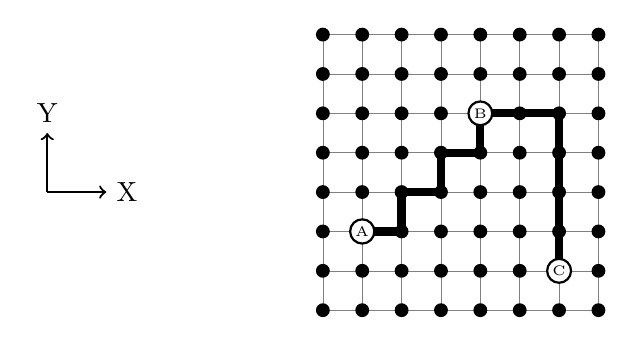
\begin{tikzpicture}[thick, scale=0.5]
	\pgfmathtruncatemacro{\width}{8}
	\pgfmathtruncatemacro{\height}{8}
	
	% Links
	\begin{scope}[help lines]
		\foreach \x in {1,...,\width}{
			\foreach [count=\y] \yy in {2,...,\height}{
				\draw (\x, \y) -- (\x, \yy);
			}
		}
		\foreach \y in {1,...,\height}{
			\foreach [count=\x] \xx in {2,...,\width}{
				\draw (\x, \y) -- (\xx, \y);
			}
		}
	\end{scope}
	
	% Nodes
	\foreach \x in {1,...,\width}{
		\foreach \y in {1,...,\height}{
			\node (node\x\y)
			      [ fill
			      , circle
			      , minimum size=0.5em
			      , inner sep=0
			      ]
			      at (\x, \y)
			      {};
		}
	}
	
	% Axes
	\coordinate (axes) at (-6, \height/2);
	\draw [->] (axes) -- ++(1.5, 0) node [anchor=west]  {X};
	\draw [->] (axes) -- ++(0, 1.5) node [anchor=south] {Y};
	
	% Route A->B
	\draw [line width=0.3em]
	      (2, 3) --
	    ++(1, 0) --
	    ++(0, 1) --
	    ++(1, 0) --
	    ++(0, 1) --
	    ++(1, 0) --
	    ++(0, 1);
	
	% Route B->C
	\draw [line width=0.3em]
	      (5, 6) --
	    ++(2, 0) --
	    ++(0, -4);
	
	% Annotations
	\foreach \x/\y/\lab in {2/3/A,5/6/B,7/2/C}{
		\node [ draw=black
		      , fill=white
		      , font=\tiny
		      , circle
		      , inner sep=0.1em
		      ]
		      at (node\x\y)
		      {\lab};
	}
\end{tikzpicture}
